% Explanation of the Provided Design

Create a new project in the same manner as in Lab 1. Manually add the provided PWM module and top level files alongside their associated simulation and constraints files. Ensure that the correct file is listed as the top level and generate the associated bit stream file. 
\begin{figure}[H]
    \centering
    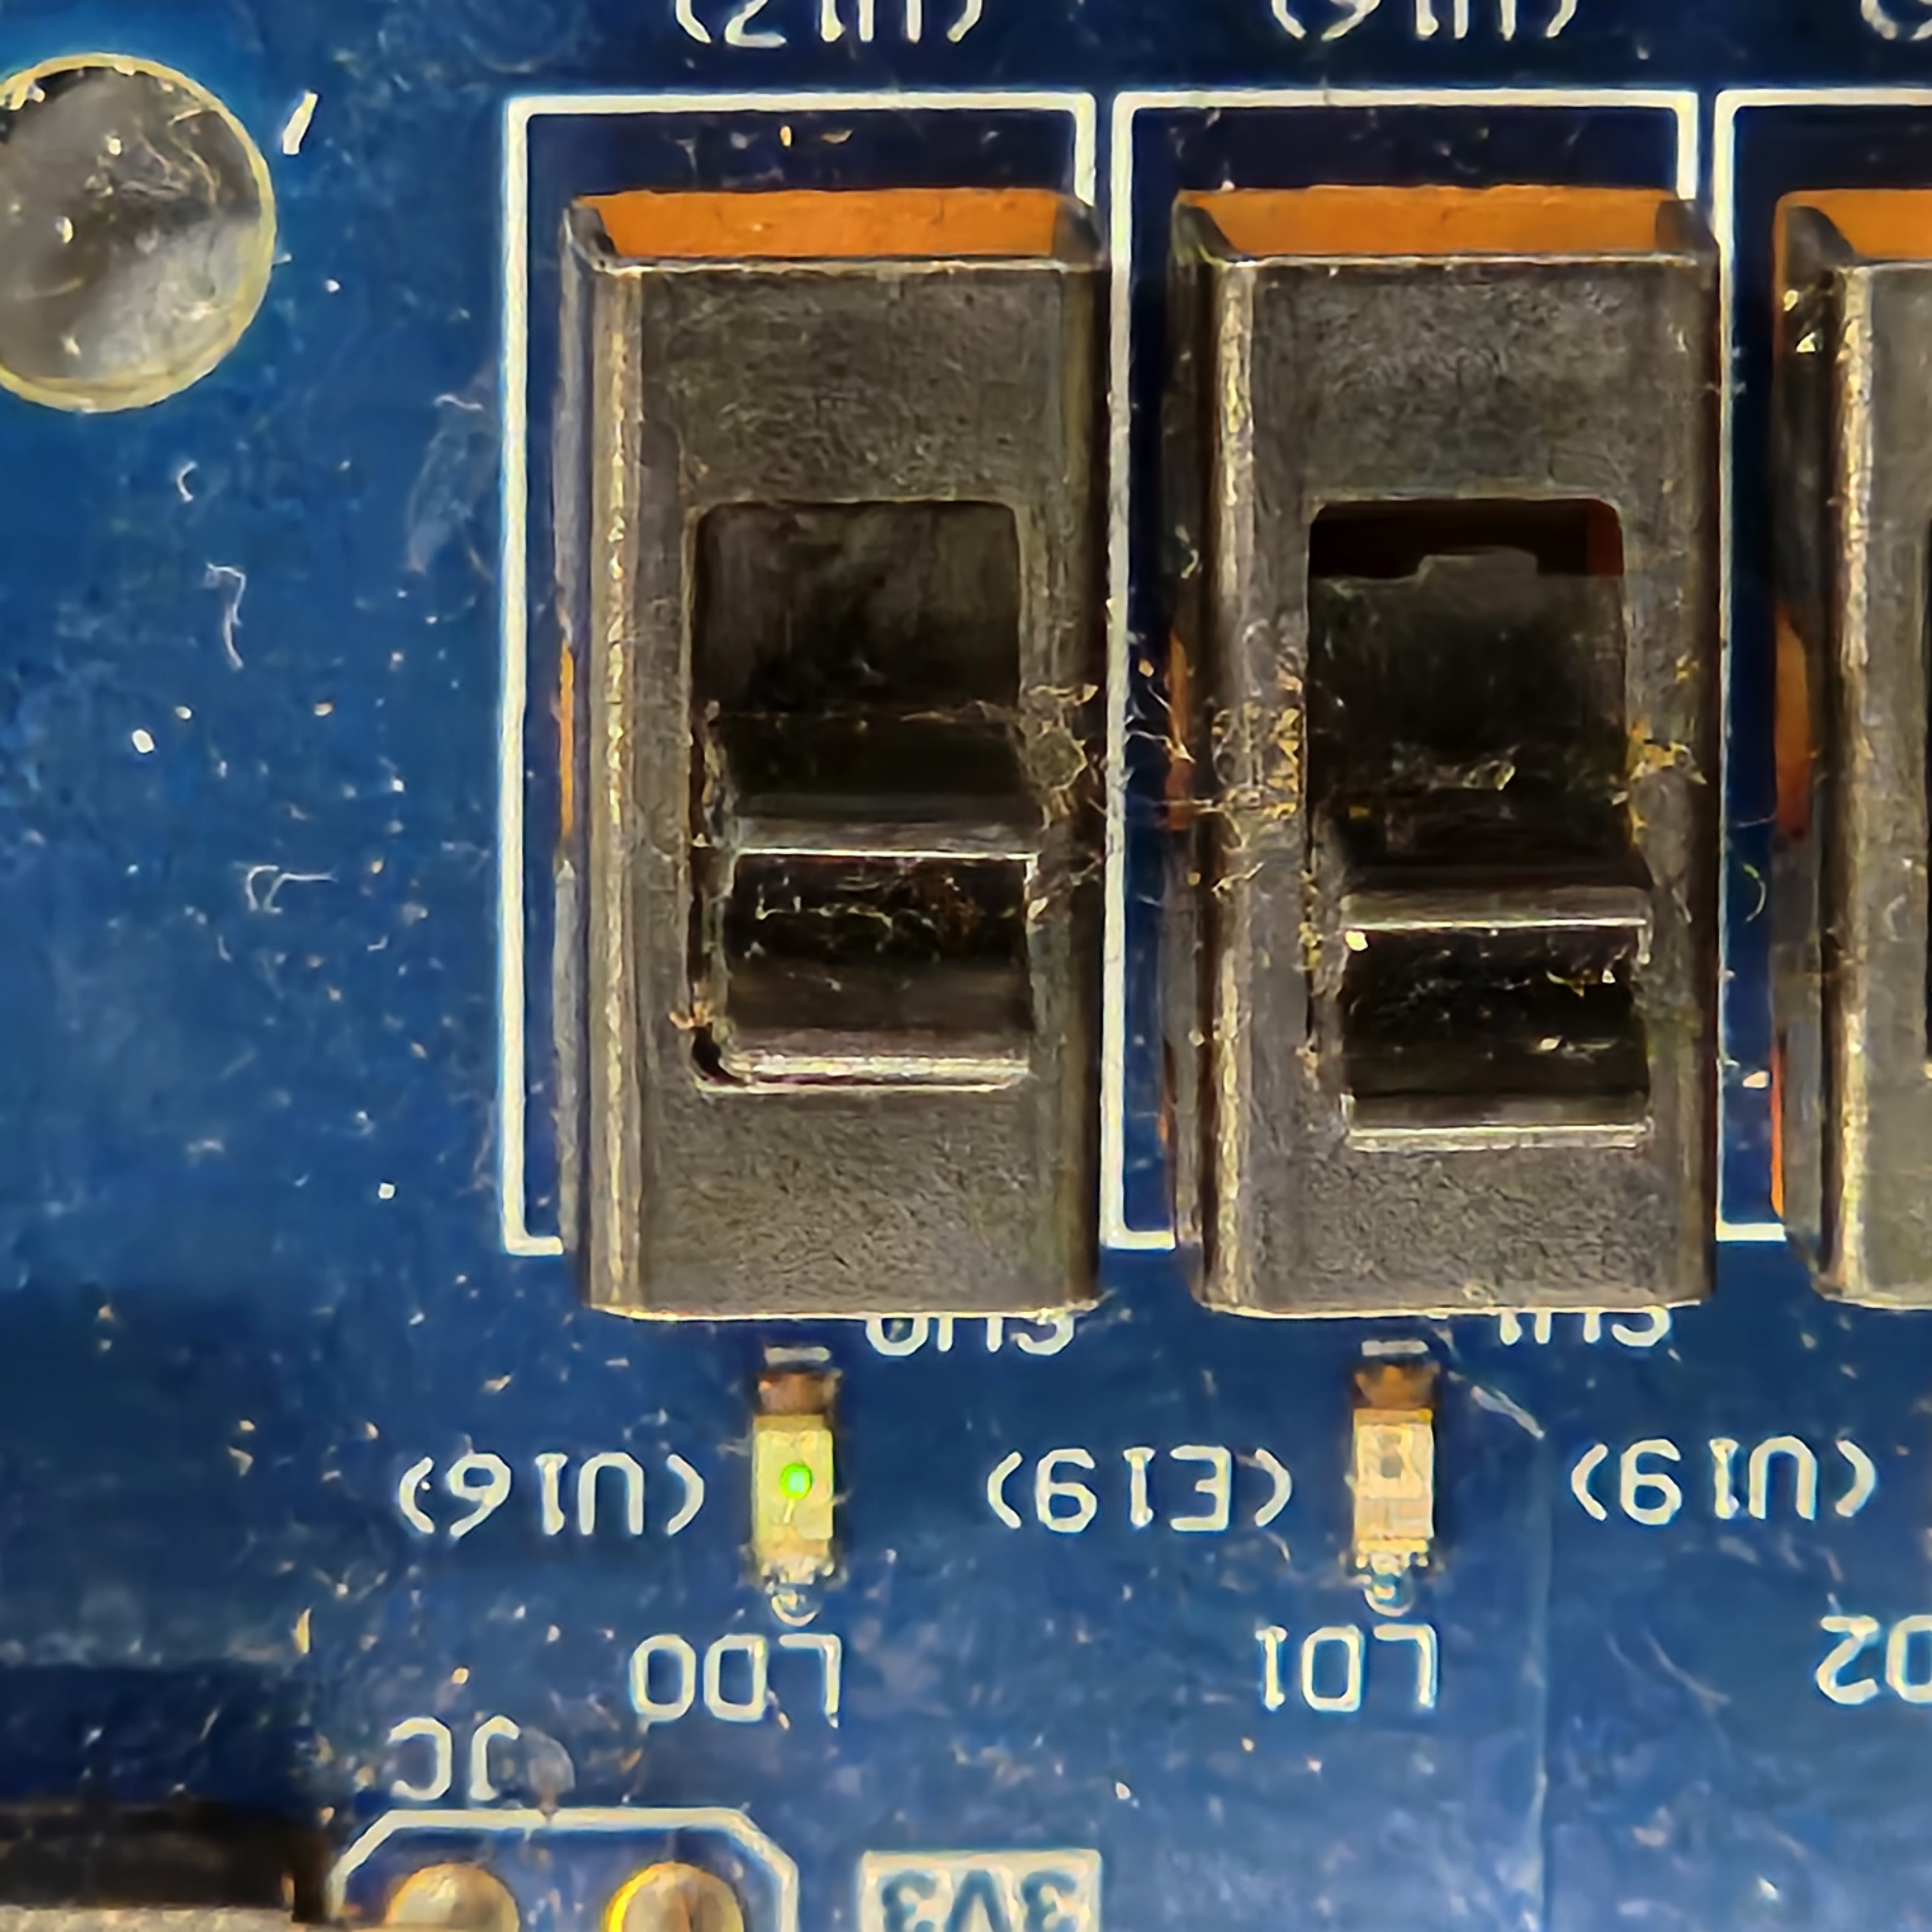
\includegraphics[width = 7cm, angle = 180]{Images/ProvidedPWM/PWM_HardwareTest.jpg}
    \caption{Provided Code Compiled onto the Basys 3}
    \label{fig:enter-label}
\end{figure}
If you were able to upload the code to the Basys 3 this is the very basic functionality which the code currently completes. One LED is controlled with its brightness being set by the associated switches. Assuming you are completing this in advance of the lab session, run the top level simulation to see this behavior shown in the simulations.
\vspace{0.5cm}
\begin{figure}[H]
    \centering
    \includemovie{1cm}{1cm}{Images/ProvidedPWM/Single_Led_Output.gif}
    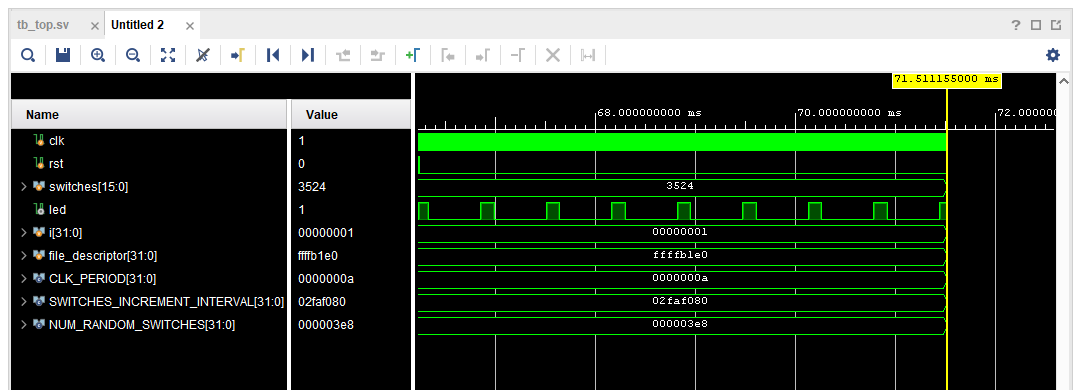
\includegraphics[width = 7cm]{Images/ProvidedPWM/Vivado_Simulate_Lab2_PWM_Module.png}
    \caption{Provided Code Simulation Results}
    \label{fig:enter-label}
\end{figure}
The top level simulation which is intended to test the functionality of the design overall does the following things: 
\begin{itemize}
    \item Starts a 100MHz Clock to match the System Clock
    \item Sets all the switches to 0
    \item Sets the RST to High for 2 Clock Cycles
    \item Watches for some time
    \item Randomizes the switch value and watches again. Repeating indefinitely. 

\end{itemize}

Looking in the wave window at the PWM\_OUT you should see the duty cycle adjusting randomly. The lower level testbenches already served to verify the functionaltiy of the PWM module so this top level one serves to verify the functionality of the system as a whole. To this end if you look in your directory after running the simulation for some time you should see a neew textfile has been created \textit{leds.txt}, this file recorded all the LED value changes alongside their times. We've prepared a tool to allow you to see the led output before being in the lab. We'll go into how this tool works and how to use it in more detail in the next section.    